\documentclass[../main.tex]{subfiles}

\begin{document}
\chapter{Two Body Particle Kinematics}
In this chapter the two body particle kinematics required to generate the multigroup charged particle data are derived. The general two body collision is described in the laboratory (LAB) and center of mass (CM) frame of references is shown in Figure \ref{fig:two-body-figure}. 
\begin{figure}[!htb]
  \centering
  \begin{subfigure}{.45\textwidth}
    \centering
    \includegraphics[scale=0.75]{../figs/twobodylab.pdf}
    \caption{LAB frame}
    \label{fig:lab-fom}
  \end{subfigure}%
  \begin{subfigure}{.45\textwidth}
    \centering
    \includegraphics[scale=0.75]{../figs/twobodycm.pdf}
    \caption{CM frame}
    \label{fig:cm-fom}
  \end{subfigure}
  \caption{A two-body collision in the laboratory (LAB) and center of mass (CM) frames of reference}
  \label{fig:two-body-figure}
\end{figure}
In Figure \ref{fig:two-body-figure} the general description of the reaction is an an incident particle of mass $m_1$ and LAB velocity $v_1$ colliding with a target particle of mass $m_2$ and zero initial velocity. This collision produces two particles which are emitted with velocities $v_3$ and $v_4$ and scattered through angles $\theta$ and $\phi$. The lighter particle has mass $m_3$ and is referred to as the scattered particle while the heavier particle with mass $m_4$ is called the recoil particle. If the identity of the outgoing particles differs from the initial particles the reaction is said to be a nuclear reaction collision and will have a $Q$-value associated with it. This $Q$-value describes the amount of energy absorbed or released during the nuclear reaction.

In the remainder of this chapter several relationships that will be useful to compute the multigroup charged particle data are derived. The first relationship describes how incident and scattered particles laboratory (LAB) energies are related to the LAB scattering angle. This relationship is then examined to determine the limits on in both angle and energy into which the scattered and recoil particles can be scattered into. Next a relationship between the CM and LAB scattering angles is derived. Finally, the relationships necessary to transform a collision from the typical target frame of reference into the incident particles frame reference are derived.


\section{Energy-angle relationship}
To derive a relationship between the laboratory scattering angle $(\theta)$, the incident particle energy $(E_1)$, and the scattered particle's energy $(E_3)$, the energy conservation equation for the general two-body reaction is expressed as
\begin{equation}
  E_{1} = E_{3} + E_{4} - Q,
\end{equation}
where $Q$ is the energy released in the reaction. Solving for $E_{4}$ gives
\begin{equation} \label{eqn:energy4-expression}
  E_{4} = E_{1} - E_{3} + Q.
\end{equation}
Using the conservation of momentum in the y-direction,
\begin{equation}
  0 = m_{3} \, v_{3} \sin \theta + m_{4} \, v_{4} \sin \phi,
\end{equation}
squaring the equation and using trigonometry identities,
\begin{equation} \label{eqn:cos_phi_1}
  \cos \phi = \sqrt{1 - \dfrac{m_{3}^2 \, v_{3}^2}{m_{4}^2 \, v_{4}^2} (1 - \cos^2 \theta)}.
\end{equation}
Next, using momentum balance in the x-direction,
\begin{equation}
  m_{1} v_{1} = m_{3} v_{3} \cos \theta + m_{4} v_{4} \cos \phi,
\end{equation}
and substituting in Eq. \eqref{eqn:cos_phi_1} gives
\begin{equation} \label{eqn:relationship-1}
  \cos \theta \sqrt{m_{1} m_{3} E_{1} E_{3}} =  \dfrac{1}{2} \left[m_{1} E_{1} + m_{3} E_{3} - m_{4} E_{4}\right].
\end{equation}
Finally, substituting Eq. \eqref{eqn:energy4-expression} into Eq. \eqref{eqn:relationship-1} gives a relationship between the cosine of the LAB scattering angle and the incident and scattered LAB energies, that is,
\begin{equation} \label{eqn:two-body-kinematics}
  \cos \theta = \mu = \dfrac{1}{2} \Bigg[\frac{m_{1} - m_{4}}{\sqrt{m_{1} \, m_{3}}}\sqrt{\dfrac{E_{1}}{E_{3}}} + \frac{m_{3} + m_{4}}{\sqrt{m_{1} \, m_{3}}}\sqrt{\dfrac{E_{3}}{E_{1}}} - \dfrac{m_{4} \, Q}{\sqrt{m_{1} m_{3} E_{1} E_{3}}}\Bigg].
\end{equation}

Similarly, a relationship can be derived for the recoil scattering angle $\phi$, the incident particles energy $E_1$, and the recoil particles energy $E_4$. Doing so gives the following relationship,
\begin{equation} \label{eqn:recoil-two-body-kinematics}
  \cos \phi = \eta = \dfrac{1}{2} \Bigg[\frac{m_{1} - m_{3}}{\sqrt{m_{1} \, m_{4}}}\sqrt{\dfrac{E_{1}}{E_{4}}} + \frac{m_{3} + m_{4}}{\sqrt{m_{1} \, m_{4}}}\sqrt{\dfrac{E_{4}}{E_{1}}} - \dfrac{m_{3} \, Q}{\sqrt{m_{1} m_{4} E_{1} E_{4}}}\Bigg].
\end{equation}
Note that Eq. \eqref{eqn:recoil-two-body-kinematics} is simply Eq. \eqref{eqn:two-body-kinematics} with particles $(3)$ and $(4)$ switched, meaning that the same kinematic relationship can be used for both the scattered particle and the recoil particle if the appropriate masses and energies are used. For example to get the cosine of the recoil scattering angle $\eta$ from Eq. \eqref{eqn:two-body-kinematics}, simply set $E_3$ to the recoil particles energy, $m_3$ to the recoil particles mass, and $m_4$ to the scattered particles mass.

In the remainder of this section Eqs. \eqref{eqn:two-body-kinematics} and \eqref{eqn:recoil-two-body-kinematics} are examined for both elastic scattering collisions, and nuclear reaction collisions. This examination is done by plotting either the cosine of the scattering or recoil angles versus the outgoing scattered or recoil particle energies for various incident energies. This examination will highlight the behavior and limits of Eqs. \eqref{eqn:two-body-kinematics} and \eqref{eqn:recoil-two-body-kinematics} for all types of collisions.

\subsection{Elastic scattering collisions}
In an elastic scattering collision the energy-angle relationship (Eq. \ref{eqn:two-body-kinematics}) can be simplified due to the fact that the outgoing particles are identical in mass to the incident and target particles, and therefore the reaction releases no energy, that is, $m_{3} = m_{1}$, $m_{4} = m_{2}$, and $Q = 0$. Substituting these properties of elastic scattering, Eq. \eqref{eqn:two-body-kinematics} reduces to 
\begin{equation} \label{eqn:elastic-scattering-angle-energy-rel}
  \mu = \dfrac{1}{2} \left[\left(1 - A\right)\sqrt{\dfrac{E_{1}}{E_{3}}} + \left(1 + A\right)\sqrt{\dfrac{E_{3}}{E_{1}}}\right], \quad A = \dfrac{m_{2}}{m_{1}},
\end{equation}
and Eq. \eqref{eqn:recoil-two-body-kinematics} reduces to 
\begin{equation} \label{eqn:elastic-recoil-angle-energy-rel}
  \eta = \dfrac{(1+A)}{2 \sqrt{A}} \sqrt{\dfrac{E_4}{E_1}}, \quad A = \dfrac{m_{2}}{m_{1}}.
\end{equation}

Additionally, there are three different types of collisions that occur: 1) light collision, 2) heavy collision, 3) identical particle collision. In light collisions the incident particle is lighter in mass than the target particle. Conversely, in a heavy collision the incident particle is heavier in mass than the target particle. Finally, in an identical particle collision the incident particle is of equal mass to the target which complicates the kinematics particularly in the special case of elastic scattering where due to quantum mechanics it is impossible to distinguish which outgoing particle corresponds to the original incident and target particles.

\subsubsection{Light elastic scattering collisions}
In light-elastic scattering collisions the mass of the incident particle is less than that of the target particle. Figure \ref{fig:light-elastic-energy-angle} shows Eqs. \eqref{eqn:elastic-scattering-angle-energy-rel}  and \eqref{eqn:elastic-recoil-angle-energy-rel} for an incident particle of mass $m_1 = 2$ undergoing an elastic scattering collision with a target particle of mass $m_2 = 2$. 
\begin{figure}[!htb]
  \centering
  \begin{subfigure}{.5\textwidth}
    \centering
    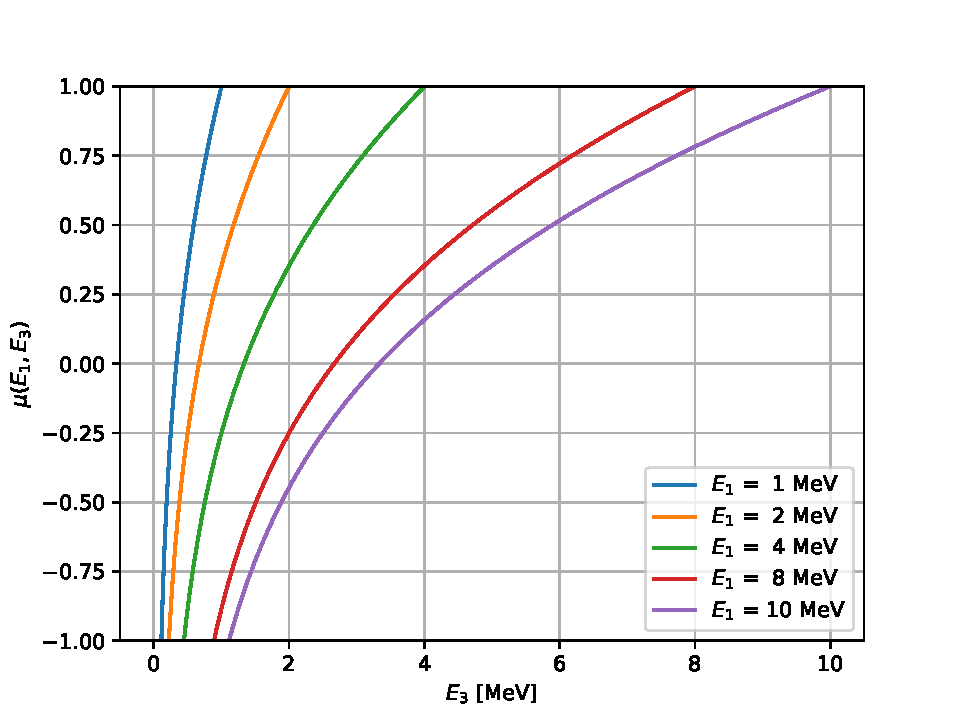
\includegraphics[width=\linewidth]{../figures/particle_kinematics/light_energy_angle.pdf}
    \caption{Scattered particle}
    \label{fig:light-elastic-energy-angle-scattered}
  \end{subfigure}%
  \begin{subfigure}{.5\textwidth}
    \centering
    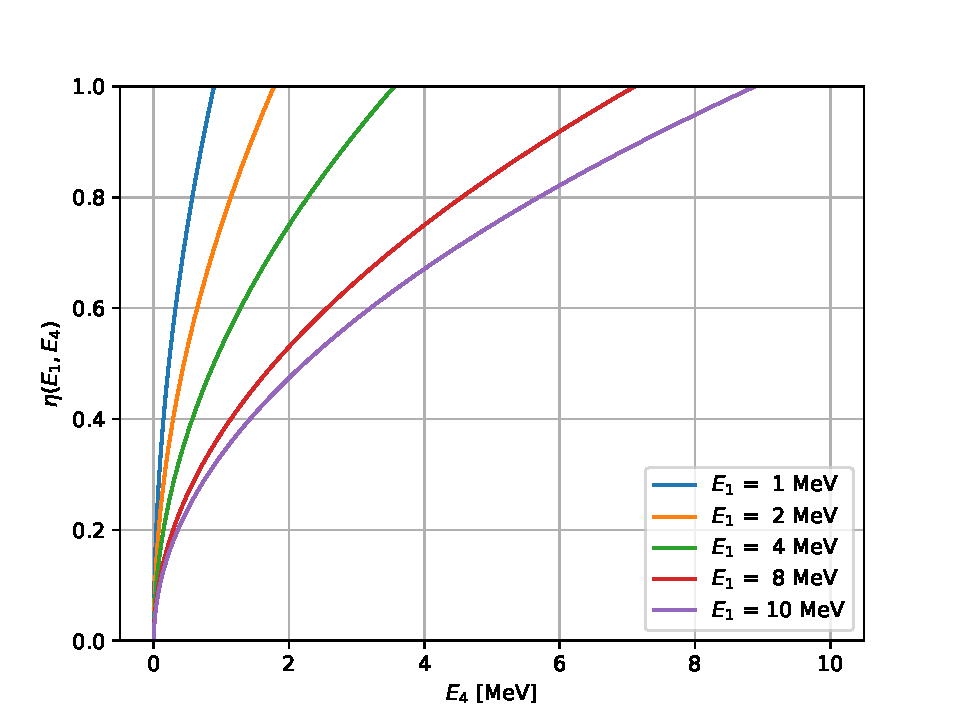
\includegraphics[width=\linewidth]{../figures/particle_kinematics/light_recoil_energy_angle.pdf}
    \caption{Recoil particle}
    \label{fig:light-elastic-energy-angle-recoil}
  \end{subfigure}
  \caption{Energy-angle relationships for both the scattered (left) and recoil (right) particles in a light elastic scattering collision where $m_1 = 2$ and $m_2 = 4$}
  \label{fig:light-elastic-energy-angle}
\end{figure}

From Figure \ref{fig:light-elastic-energy-angle} the incident particle can be scattered through all angles, $\theta \in [0^{\circ}, 180^{\circ}]$ while the target particle can only be scattered through forward angles, $\phi \in [0^{\circ}, 90^{\circ}]$. Additionally, if no collision takes place the incident particle loses no energy and the recoil particle gains no energy. To derive an expression for the maximum energy that an incident particle can lose in a light elastic collision consider that the maximum energy loss occurs when $\mu = -1$. Substituting $\mu = -1$ into Eq. \eqref{eqn:elastic-scattering-angle-energy-rel} and solving for $E_3$ gives
\begin{equation}
  E_{3,\text{min}} = \left(\dfrac{A - 1}{A + 1}\right)^2 E_1, \quad \text{where} \,\, A = \dfrac{m_2}{m_1}.
\end{equation}
Conversely the maximum energy that the recoil particle can gain is 
\begin{equation}
  E_{4,\text{max}} = \left[1 - \left(\dfrac{A - 1}{A + 1}\right)^2\right] E_1, \quad \text{where} \,\, A = \dfrac{m_2}{m_1}.
\end{equation}

\subsubsection{Heavy elastic scattering collisions}
In heavy elastic scattering collisions the mass of the incident particle is greater than the target particles mass. This results in the incident particle only being able to lose a finite amount of energy in a single collision. Figure \ref{fig:heavy-elastic-energy-angle} shows Eqs. \eqref{eqn:elastic-scattering-angle-energy-rel}  and \eqref{eqn:elastic-recoil-angle-energy-rel} for an incident particle of mass $m_1 = 2$ undergoing an elastic scattering collision with a target particle of mass $m_2 = 2$. 
\begin{figure}[!htb]
  \centering
  \begin{subfigure}{.5\textwidth}
    \centering
    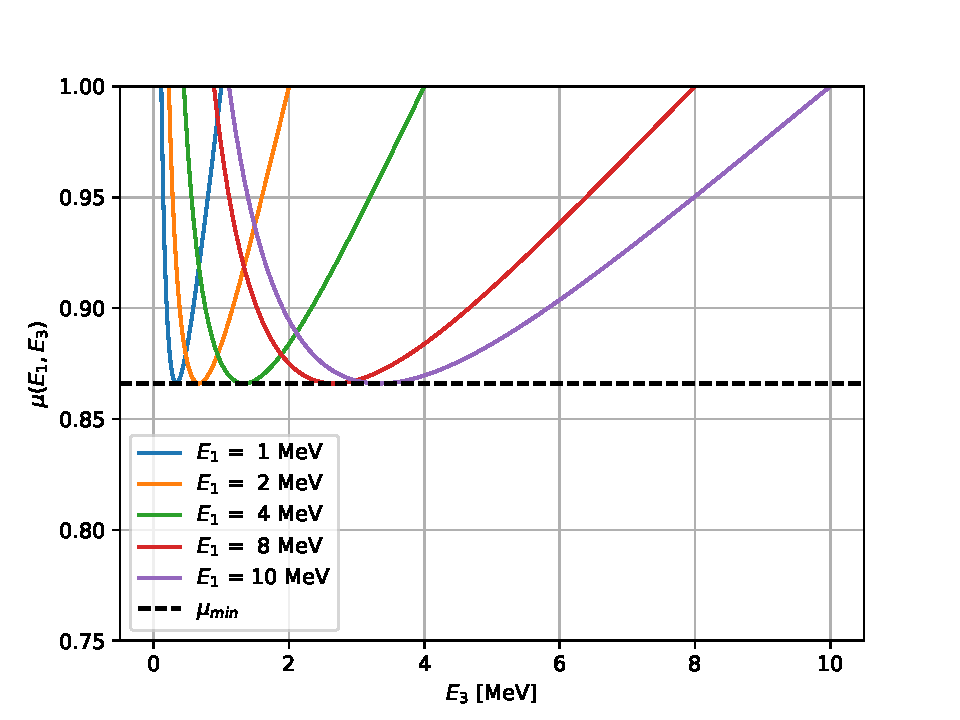
\includegraphics[width=\linewidth]{../figures/particle_kinematics/heavy_energy_angle.pdf}
    \caption{Scattered particle}
    \label{fig:heavy-elastic-energy-angle-scattered}
  \end{subfigure}%
  \begin{subfigure}{.5\textwidth}
    \centering
    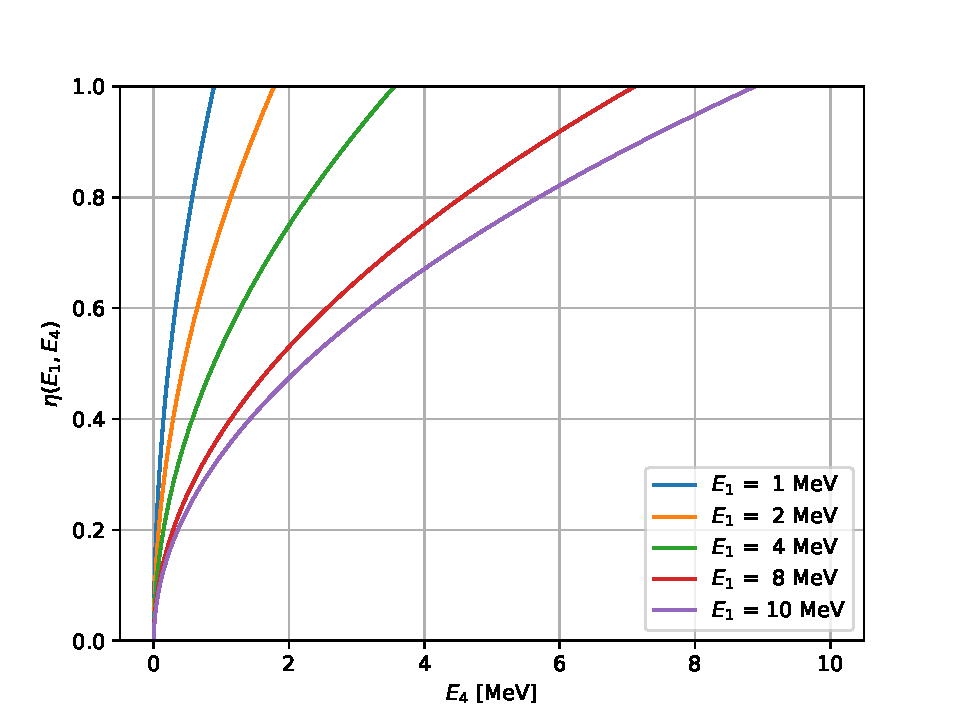
\includegraphics[width=\linewidth]{../figures/particle_kinematics/heavy_recoil_energy_angle.pdf}
    \caption{Recoil particle}
    \label{fig:heavy-elastic-energy-angle-recoil}
  \end{subfigure}
  \caption{Energy-angle relationships for both the scattered and recoil particles in a heavy elastic scattering collision where $m_1 = 2$ and $m_2 = 4$}
  \label{fig:heavy-elastic-energy-angle}
\end{figure}

From Figure \ref{fig:heavy-elastic-energy-angle} it is clear that Eq. \eqref{eqn:elastic-scattering-angle-energy-rel} has a minimum scattering angle that is independent of the incident particles energy, while the recoil particle can only scatter in the LAB frame of reference between the angles $0^{\circ}$ and $90^{\circ}$. The minimum scattering angle is found by taking the derivative of Eq. \eqref{eqn:elastic-scattering-angle-energy-rel} with respect to $E_{3}$,
\begin{equation} \label{eqn:derivative-of-mu}
  \dfrac{d \mu}{d E_{3}} = \dfrac{1}{4} \left[\left(1 + A\right)(E_{3})^{\frac{1}{2}}(E_{1})^{-\frac{1}{2}} - \left(1 - A\right)(E_{1})^{\frac{1}{2}}(E_{3})^{-\frac{3}{2}}\right].
\end{equation}
Next setting Eq. \eqref{eqn:derivative-of-mu} equal to zero and solving for $E_{3}$ gives
\begin{equation} \label{eqn:max-energy-loss}
  E_{3,\text{min}} = \dfrac{1-A}{1+A} E_{1}.
\end{equation}
Note, Eq. \eqref{eqn:max-energy-loss} is an expression for the minimum energy that an incident particle of energy $E_1$ can have after a collision. Similarly, the maximum energy that the recoil particle can have after the collision is
\begin{equation}
  E_{4,\text{max}} = \left(1 - \dfrac{1-A}{1+A}\right) E_{1}.
\end{equation}
Substituting Eq. \eqref{eqn:max-energy-loss} back into Eq. \eqref{eqn:elastic-scattering-angle-energy-rel} gives an expression for the cosine of the minimum scattering angle, that is,
\begin{equation}
  \mu_{\text{min}} = \sqrt{(1+A)(1-A)} = \Big[1 - A^2\Big]^{\frac{1}{2}}, \quad \text{for} \,\, m_{1} > m_{2}.
\end{equation}

\subsubsection{Identical elastic scattering collisions}
In identical elastic scattering collisions the mass of the incident particle is equal to the target particles mass. This results in the incident particle can lose anywhere from zero to all of its energy in a single collision. Additionally, because the collision is an elastic scattering collision the identity of the scattered and recoil particles do not change making them indistinguishable. To remedy this the more energetic outgoing particle is assumed to be the scattered particle while the less energetic particle is considered to be the recoil particle. The energy-angle relationships given by Eqs. \eqref{eqn:elastic-scattering-angle-energy-rel}  and \eqref{eqn:elastic-recoil-angle-energy-rel} reduce to
\begin{equation}
  \mu = \sqrt{\dfrac{E_3}{E_1}}, \quad \text{and} \,\, \eta = \sqrt{\dfrac{E_4}{E_1}}.
\end{equation}
\begin{figure}[!htb]
  \centering
  \begin{subfigure}{.5\textwidth}
    \centering
    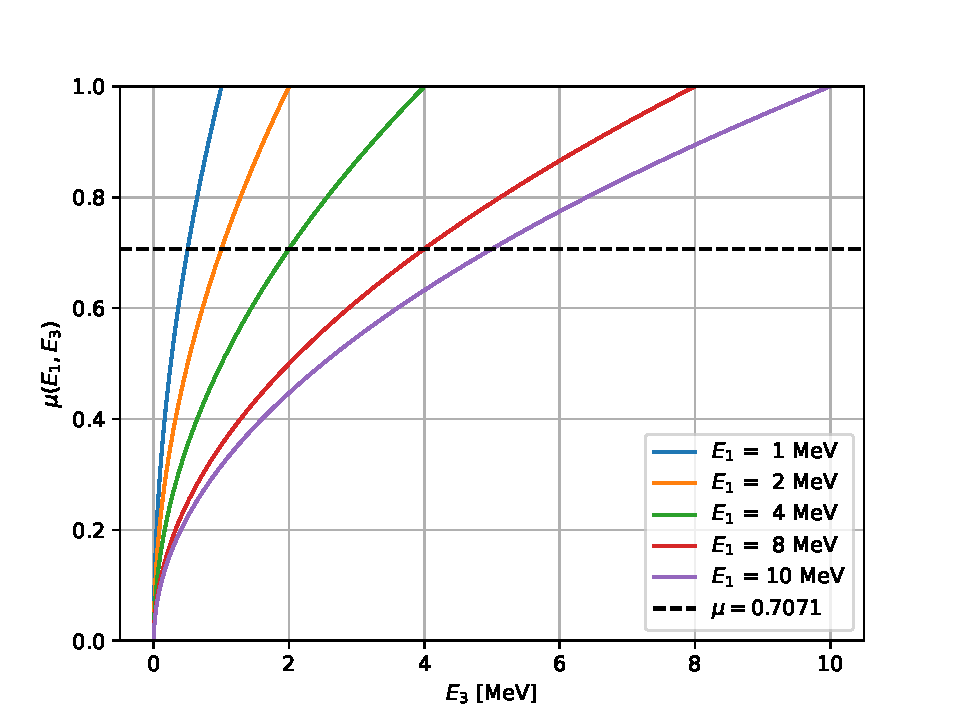
\includegraphics[width=\linewidth]{../figures/particle_kinematics/identical_energy_angle.pdf}
    \caption{Scattered particle}
    \label{fig:identical-elastic-energy-angle-scattered}
  \end{subfigure}%
  \begin{subfigure}{.5\textwidth}
    \centering
    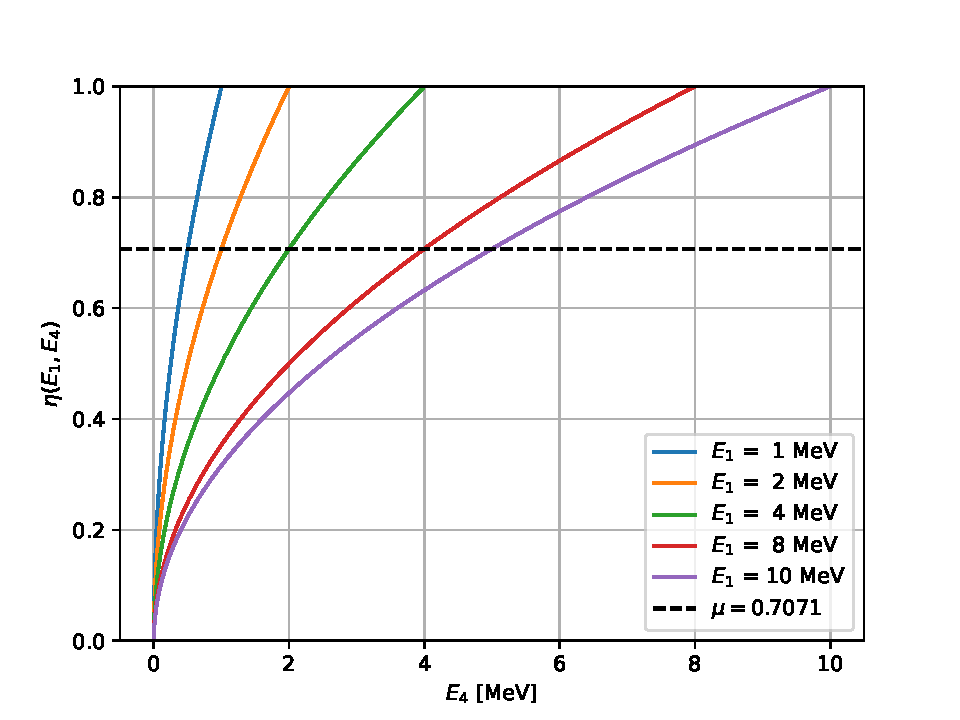
\includegraphics[width=\linewidth]{../figures/particle_kinematics/identical_recoil_energy_angle.pdf}
    \caption{Recoil particle}
    \label{fig:identical-elastic-energy-angle-recoil}
  \end{subfigure}
  \caption{Energy-angle relationships for both the scattered and recoil particles in an identical particle elastic scattering collision where $m_1 = 2$ and $m_2 = 2$}
  \label{fig:identical-elastic-energy-angle}
\end{figure}

In an identical particle elastic scattering event it is impossible to differentiate between the incident and the recoil particles, therefore the convention adopted is to take the scattered particle to be the more energetic particle while the less energetic particle to be the recoil particle. This energy cutoff used to differentiate between the particles is found by considering any particle with outgoing energy greater than half the initial energy to be the scattered particle. This energy cutoff corresponds to a cutoff angle in LAB frame, that is,
\begin{equation}
  \mu_{\text{cut}} = \sqrt{\dfrac{\frac{1}{2} E_1}{E_1}} = \dfrac{\sqrt{2}}{2} \approx 0.7071.
\end{equation}
From Figure \ref{fig:identical-elastic-energy-angle} the energy-angle relationship for both the scattered and recoiling particles are identical because the masses are identical. The only distinguishing feature between the scattered and recoiling particles is that in Figure \ref{fig:identical-elastic-energy-angle-scattered} any particle scattered into a cosine of scattering angle less than $\mu_{\text{cut}}$ (i.e. below dashed line) is considered a recoil particle. Conversely, in Figure \ref{fig:identical-elastic-energy-angle-recoil} any particle scattered into a cosine of scattering angle greater than $\mu_{\text{cut}}$ (i.e. above dashed line) is considered a scattered particle.

\subsection{Nuclear reaction collisions}
In nuclear reaction collisions the identities of the incident and target particles change as a result of the reaction. Additionally, because the masses of the particles the reaction release energy denoted as $Q$. Figure \ref{fig:nuclear-reaction} shows Eqs. \eqref{eqn:two-body-kinematics} and \eqref{eqn:recoil-two-body-kinematics} for the reaction $\text{T}(d,n)\text{He-4}$.
\begin{figure}[!htb]
  \centering
  \begin{subfigure}{.5\textwidth}
    \centering
    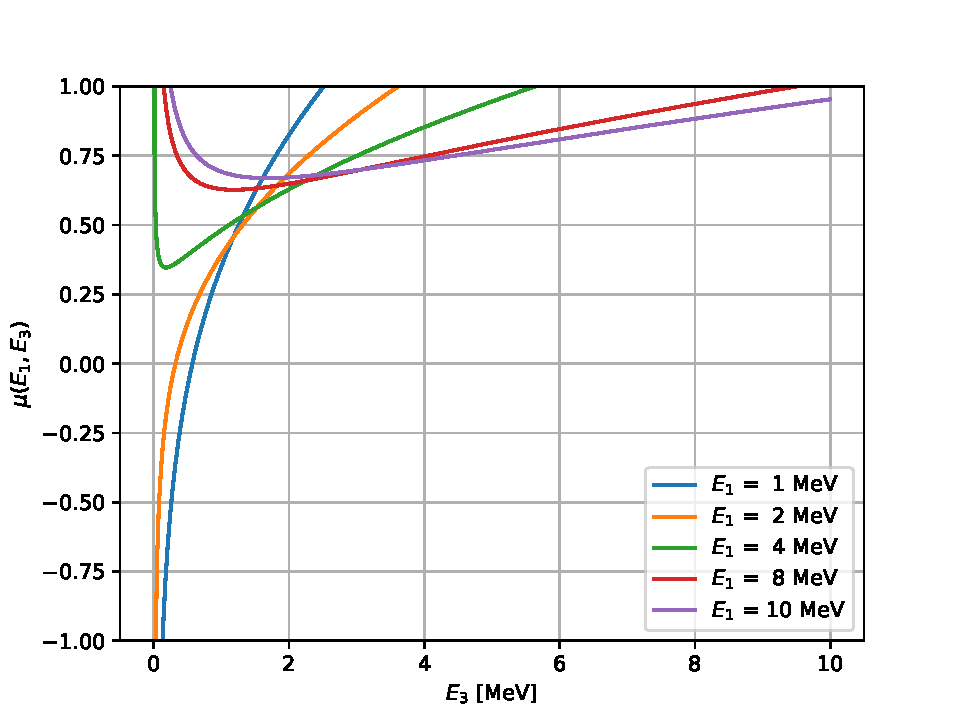
\includegraphics[width=\linewidth]{../figures/particle_kinematics/light_rx_energy_angle.pdf}
    \caption{Scattered particle}
    \label{fig:nuclear-reaction-scattered}
  \end{subfigure}%
  \begin{subfigure}{.5\textwidth}
    \centering
    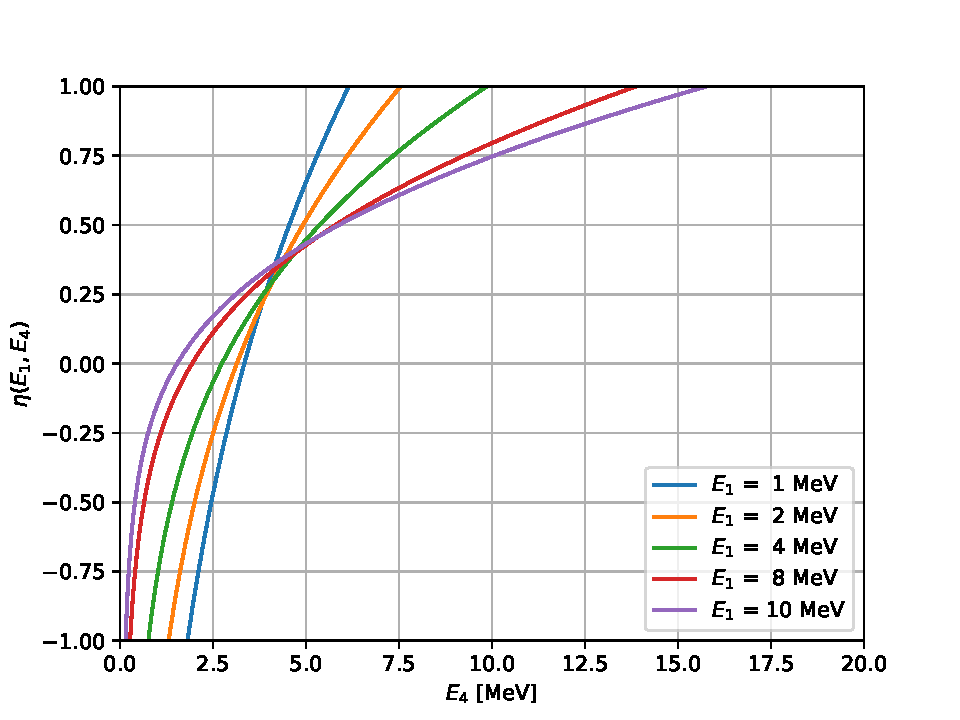
\includegraphics[width=\linewidth]{../figures/particle_kinematics/light_rx_recoil_energy_angle.pdf}
    \caption{Recoil particle}
    \label{fig:nuclear-reaction-recoil}
  \end{subfigure}
  \caption{Energy-angle relationships for both the scattered and recoil particles in the nuclear reaction collision $\text{T}(d,n)\text{He-4}$}
  \label{fig:nuclear-reaction}
\end{figure}

From Figure \ref{fig:nuclear-reaction} both the scattered and recoil particles can scatter through all possible scattering and recoil angles $\theta \in [0^{\circ}, 180^{\circ}]$ and $\phi \in [0^{\circ}, 180^{\circ}]$. This is because the incident and target particles combine to form a compound nucleus and then break apart into two different products. The minimum and maximum energies that the scattered particle can have after a reaction occur at cosine of scattering angles of $-1$ and $1$ as depicted by Figure \ref{fig:nuclear-reaction-scattered} and are
\begin{equation}
  E_{3,\text{min}} = E_3^C - 2 \sqrt{k_3 \, E_3^C \, E_1} + k_3 E_1, \quad E_{3,\text{max}} = E_3^C + 2 \sqrt{k_3 \, E_3^C \, E_1} + k_3 E_1
\end{equation}
where $k_3 = m_1 m_3 / (m_1+m_2)^2$, and $E_3^C$ is the energy in the CM frame of reference of the scattered particle (this expression is derived in the section). Similarly, the maximum and minimum energies of the recoil particle are
\begin{equation}
  E_{4,\text{min}} = E_4^C - 2 \sqrt{k_4 \, E_4^C \, E_1} + k_4 E_1, \quad E_{4,\text{max}} = E_4^C + 2 \sqrt{k_4 \, E_4^C \, E_1} + k_4 E_1
\end{equation}
where $k_3 = m_1 m_3 / (m_1+m_2)^2$, and $E_3^C$ is the energy in the CM frame of reference of the scattered particle (this expression is derived in the section).

\subsection{Energy-angle relationships summary}
Here the energy and angle limits derived in the previous sections are summarized as to provide a location to quickly refer back to. Table \ref{tab:particle-kinematics} lists the minimum and maximum scattering angles and energies for both the scattered and recoil particles for all types of two body collisions. From Table \ref{tab:particle-kinematics} only in light elastic and nuclear reaction collisions can the scattered particle scatter through all possible scattering angles. Additionally, in all elastic scattering collisions the recoil particle can have anywhere from zero to some maximum amount of energy as defined by the particle kinematics.
\begin{table}[!htb]
  \centering
  \caption{Summary of the limits on the energy-angle relationships for all possible types of two-body collisions}
  \label{tab:particle-kinematics}
  \begin{tabular}{c|c|c|c|c}
  \hline
              & Light Elastic & Heavy Elastic & Identical Elastic & Nuclear Reaction \\ \hline
  $\mu_{\text{min}}$ & -1 & $1 / \alpha$ & $\sqrt{2}/2$ & -1 \\
  $\mu_{\text{max}}$ & 1 & 1 & 1 & 1 \\
  $\eta_{\text{min}}$ & 0 & 0 & 0 & -1 \\
  $\eta_{\text{max}}$ & 1 & $1 / \alpha$ & $\sqrt{2}/2$ & 1 \\
  $E_{3,\text{min}}$  & $\alpha^2 E_1$ & $-\alpha E_{1}$ & $E_1/2$ & $E_3^C - 2 \sqrt{k_3 \, E_3^C \, E_1} + k_3 E_1$ \\
  $E_{3,\text{max}}$  & $E_1$ & $E_1$ & $E_1$ & $E_3^C + 2 \sqrt{k_3 \, E_3^C \, E_1} + k_3 E_1$ \\
  $E_{4,\text{min}}$  & 0 & 0 & 0 & $E_4^C - 2 \sqrt{k_4 \, E_4^C \, E_1} + k_4 E_1$ \\
  $E_{4,\text{max}}$  & $\left(1 - \alpha^2\right) E_1$ & $\left(1 + \alpha\right) E_{1}$ & $E_1 / 2$ & $E_4^C + 2 \sqrt{k_4 \, E_4^C \, E_1} + k_4 E_1$ \\ \hline
  \end{tabular}
\end{table}

% ------------------------------------------------------------------------------
% ------------------------------------------------------------------------------
\section{Laboratory and center of mass relationships}
The next relationship that will be useful to compute the multigroup charged particle data is a relationship between the center of mass and laboratory cosine of scattering angles. This relationship is found by considering the diagram in Figure \ref{fig:lab_com_rel}.
\begin{figure}[!htb]
  \centering
  \includegraphics{../figs/lab_com_relationship.pdf}
  \caption{Relationship between the CM and LAB scattering angles}
  \label{fig:lab_com_rel}
\end{figure}
In Figure \ref{fig:lab_com_rel} the superscripts $L$ and $C$ represent components in the LAB and CM reference frames, and $V_{\scaleto{CM}{3pt}}$ is the CM velocity of the two body system.

From Figure \ref{fig:lab_com_rel}, the y and x-direction velocity components are
\begin{equation}
  v_{3}^L \sin \theta_{\scaleto{L}{3pt}} = v_{3}^C \sin \theta_{\scaleto{C}{3pt}}, \quad v_{3}^L \cos \theta_{\scaleto{L}{3pt}} = v_{CM} + v_{3}^C \cos \theta_{\scaleto{C}{3pt}}.
\end{equation}
Dividing the y-direction velocity components by the x-direction velocity components gives
\begin{equation} \label{eqn:cosine-0}
  \tan \theta_L = \dfrac{\sin \theta_C}{\gamma + \cos \theta_C},
\end{equation}
where $\gamma$ is the ratio of the CM velocity of the system to the CM velocity of the outgoing particle. Squaring Eq. \eqref{eqn:cosine-0} to remove the singularity in $\tan x$ as $x \rightarrow \pi/2$ and solving for $\cos \theta_{\scaleto{C}{3pt}}$ yields the following relationship between the CM and LAB cosine of scattering angles
\begin{equation} \label{eqn:lab-com-angle-relationship}
  \mu_C = \gamma (\mu_L^2 - 1) + \mu_L \sqrt{1 + \gamma^2(\mu_L^2-1)}
\end{equation}
For Eq. \eqref{eqn:lab-com-angle-relationship} to be a meaningful relationship the value of $\gamma$ must remain positive and less than 1. Figure \ref{fig:cm-lab-cosine-relationship} shows Eq. \eqref{eqn:lab-com-angle-relationship} for several different values of $\gamma$ at all possible LAB cosine scattering angles. 
\begin{figure}[!htb]
  \centering
  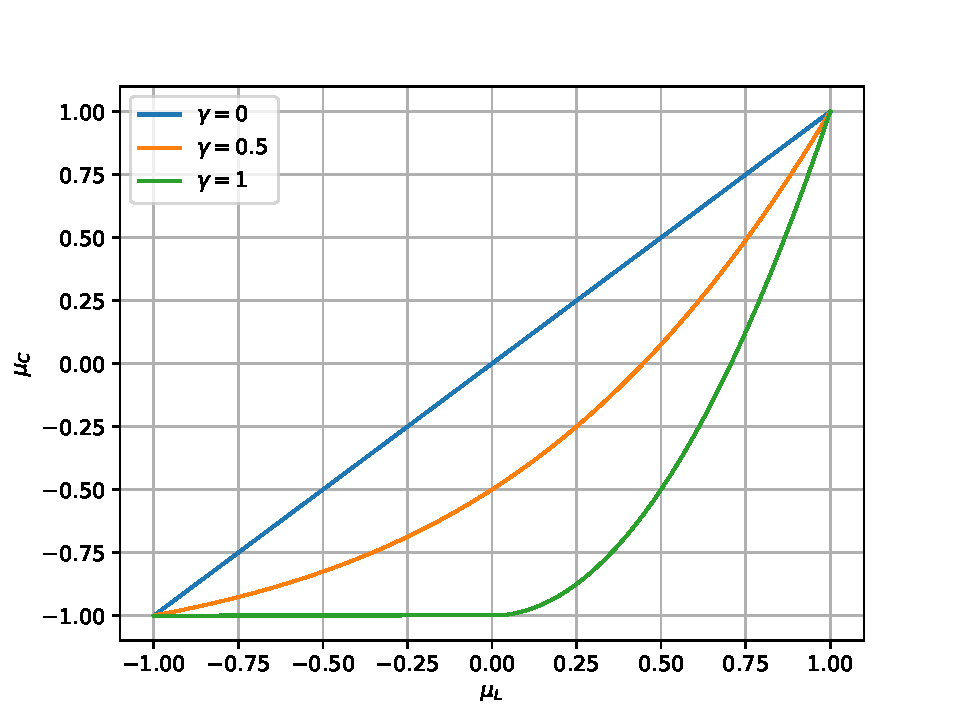
\includegraphics[scale=0.75]{../figures/particle_kinematics/cm_lab_angle_relationship.pdf}
  \caption{CM and LAB cosine of scattering angle relationship for several values of $\gamma$}
  \label{fig:cm-lab-cosine-relationship}
\end{figure}
From Figure \ref{fig:cm-lab-cosine-relationship} when $\gamma = 0$ Eq. \eqref{eqn:lab-com-angle-relationship} is linear relationship where the CM cosine angle equals the LAB angle. Then, as $\mu_L \rightarrow 1$ the relationship becomes more biased towards negative CM cosine scattering angles, that is larger positive LAB cosine angles result in negative LAB angles. The expression for $\gamma$ is derived in the next subsection.

\subsection{Center of mass and outgoing particle velocity relationship}
To determine an expression for $\gamma$ as required by Eq. \eqref{eqn:lab-com-angle-relationship} consider the CM two-body diagram shown in Figure \ref{fig:two-body-figure}. The CM velocity of the system is found by transforming the incident energy of the particle $E_1^L$ from the LAB frame to the CM frame. This is done by first considering the velocities of the projectile and target particles in the CM frame, that is,
\begin{equation} \label{eqn:cm-velocities}
    u_1 = v_1 - V, \quad u_2 = -V
\end{equation}
where $V$ is the CM velocity of the system. Next the total momentum in the CM for the system is zero, that is, the CM velocity can be solved for as
\begin{equation}
  m_1 u_1 + m_2 u_2 = 0,
\end{equation}
and by substituting Eq. \eqref{eqn:cm-velocities} into this expression give the CM velocity of the system
\begin{equation}
  V = \dfrac{m_1}{m_1 + m_2} v_1
\end{equation}

To derive an expression for the scattered particles energy in the CM, $v_3^C$, using $V$ the energy of the incident particle in the COM frame is
\begin{equation} \label{eqn:e1-cm}
  E_1^C = \dfrac{1}{2} m_1 u_1^2 = \dfrac{1}{2} m_1 \left( v_1 - \dfrac{m_1}{m_1 + m_2} v_1 \right)^2 = E_1^l \left( \dfrac{m_2}{m_1+m_2} \right)^2.
\end{equation}
Next considering the conservation of momentum,
\begin{gather} \label{eqn:momentum-blanace}
  m_1 u_1 + m_2 u_2 = 0 \implies u_2 = -\dfrac{m_1}{m_2} u_1, \\
  m_{3} u_{3} + m_{4} u_{4} = 0 \implies u_{4} = -\dfrac{m_{3}}{m_{4}} u_{3}.
\end{gather} 
From the law of conservation of energy the CM energy of the scattered particle can be written in terms of all other particle energies, that is,
\begin{equation} \label{eqn:energy-balance}
  E_1^C + E_2^C = E_3^C + E_4^C - Q \implies E_3^C = E_1^C + E_2^C - E_4^C + Q.
\end{equation}
Substituting Eq. \eqref{eqn:e1-cm} and Eq. \eqref{eqn:momentum-blanace} into Eq. \eqref{eqn:energy-balance} gives the following expression for the CM energy of the scattered particle as a function of the incident particles energy,
\begin{equation} \label{eqn:cm-scattered-velocity}
  E_{3}^C = E_1^l \left( \dfrac{m_2}{m_1+m_2} \right)^2 \left(\dfrac{m_{4}(m_2 + m_1)}{m_2(m_{4}+m_{3})}\right) + \left(\dfrac{m_{4}}{m_{4}+m_{3}}\right) Q,
\end{equation}
where $Q$ is the energy lost in a nuclear reaction. Finally, using Eq. \eqref{eqn:cm-scattered-velocity} the velocity of the outgoing particle in the CM frame is simply
\begin{equation}
  v_{3}^C = \sqrt{\frac{2 E_{3}^C}{m_{3}}}.
\end{equation}

\subsection{Jacobian}
In data sets the differential cross section are often expressed in terms of the incident particles energy in the LAB frame and the scattering angle in the CM frame. Therefore it is useful to be able to express the CM differential cross sections in the LAB frame. The differential cross section in the LAB frame of reference is written in the CM frame as
\begin{equation}
  \dfrac{\partial \sigma}{\partial \Omega^L} = \dfrac{\partial \sigma}{\partial \Omega^C} \cdot \dfrac{\sin \theta^C}{\sin \theta^L} \cdot \dfrac{\partial \theta^C}{\partial \theta^L} = \dfrac{\partial \sigma}{\partial \Omega^C} \cdot J\left(\theta^C\right)
\end{equation}
where $J(\theta^C)$ is the jacobian. Differentiating Eq. \eqref{eqn:cosine-0} gives
\begin{equation}
  \dfrac{\partial \theta^C}{\partial \theta^L} = \dfrac{\left(\gamma + \mu_C\right)^2}{\mu_L^2 \left(1 + \mu_C\right)},
\end{equation}
and the jacobian becomes
\begin{equation} \label{eqn:jacobian}
  J(\theta^C) = \dfrac{\left(\gamma + \mu_C\right)^3}{\mu_L^3 \left(1 + \mu_C\right)}
\end{equation}
where Eq. \eqref{eqn:cosine-0} was used to simplify $\sin \theta^C / \sin \theta^L$. Using Eqs. \eqref{eqn:lab-com-angle-relationship} and \eqref{eqn:jacobian} a differential cross section can be transformed from the CM frame to the LAB frame as
\begin{equation}
  \sigma(E_1,\mu_L) = \sigma[E_1, \mu_C(\mu_L)] \dfrac{\left[\gamma + \mu_C(\mu_L)\right]^3}{\mu_L^3 \left[1 + \mu_C(\mu_L)\right]},
\end{equation}
where $\mu_C$ is a function of $\mu_L$ as defined by Eq. \eqref{eqn:lab-com-angle-relationship}.

% ------------------------------------------------------------------------------
% ------------------------------------------------------------------------------
\section{Frame of Reference Transform}
Typically data files only exist for collisions where the incident particle is of less or equal mass to the target particle. To obtain the differential cross sections for collisions in which the incident particle is heavier than the target particle a simple change of reference frame is used on the inverse form of this reaction. Consider for example a high energy deuteron striking a proton at rest. Data for this reaction is typically not available; however, in the incident deuteron's frame of reference, this reaction is a high energy proton striking a deuteron at rest for which data is available. Figure \ref{fig:heavy_collisions}, shows an example of this transformation for the two body reaction.
\begin{figure}[!htb]
  \centering
  \begin{subfigure}{.45\textwidth}
    \centering
    \includegraphics[scale=0.75]{../figs/targetFOM.pdf}
    \caption{Target particle's reference frame}
  \end{subfigure}%
  \begin{subfigure}{.45\textwidth}
    \centering
    \includegraphics[scale=0.75]{../figs/incidentFOM.pdf}
    \caption{Incident particle's reference frame}
    \label{fig:sub2}
  \end{subfigure}
  \caption{Frame of reference transformation for a two-body system}
  \label{fig:heavy_collisions}
\end{figure}

To derive the expression needed to shift the frame of reference to the target particle, the velocity of the incident particle with respect to the target is
\begin{equation}
    v_1 = \sqrt{\dfrac{2 \, E_1}{m_1}},
\end{equation}
and the velocity of the target particle in the incident particle's frame of reference is
\begin{equation} \label{eqn:transform-incident-fom}
    v_2^H = -v_1,
\end{equation}
where the superscript $H$ represents a transformation to the incident particles frame of reference. Using Eq. \eqref{eqn:transform-incident-fom}, the target particle's energy in the incident particle's frame of reference is
\begin{equation} \label{eqn:frame_shift}
    E_2^H = \dfrac{1}{2} \, m_2 \, (v_2^H)^2 = \left( \dfrac{m_2}{m_1} \right) E_1.
\end{equation}
Using Eq. \ref{eqn:frame_shift} the differential cross sections for the heavy on light reaction can be expressed in terms of the differential cross section for the corresponding light on heavy reaction as
\begin{equation}
  \sigma_{1 \rightarrow 2}(E_p^L,\mu_0) = \sigma_{2 \rightarrow 1}(E_t^H,\mu_0).
\end{equation}

Lastly, to compute the Fokker-Planck moments of the differential cross section for the heavy on light from the corresponding light-on-heavy reactions an additional transform is required due to the Jacobian that appears when transforming the integral accordingly. The Fokker-Planck coefficients for the heavy-on-light reaction in terms of the light-on-heavy reaction are
\begin{equation}
  F^{k,j}(E_1) = \left(\dfrac{E_1}{E_2^H}\right)^k F^{k,j}(E_2^H) = \left(\dfrac{m_1}{m_2}\right)^k F^{k,j}(E_2^H).
\end{equation}

\end{document}